\documentclass{article}
\usepackage[english]{babel}
\usepackage[letterpaper,top=2cm,bottom=2cm,left=3cm,right=3cm,marginparwidth=1.75cm]{geometry}
\usepackage{amsmath}
\usepackage{graphicx}
\usepackage[colorlinks=true, allcolors=blue]{hyperref}
\usepackage[numbers]{natbib}
\usepackage{listings}

\title{NOvA Production 6 Validation Task Force Contribution Summary}
\author{Oscar Chow}

\begin{document}
\maketitle

\section{Task Description}
I contributed to the Production 6 Validations for variables at both the ND and FD.
I looked at the $\nu_{\mu}$ side at the ND and both the $\nu_{\mu}$ and $\nu_e$ sides at the FD.
A summary of my contributions is given below.

\subsection{ND: \texorpdfstring{$\nu_\mu$}{numu} MC to MC Comparisons \& PID cut retuning}
\label{sec:nd-numu}
My work on the ND $\nu_{\mu}$ side was captured in three talks~\cite{ochow-nd-numu-init,ochow-nd-numu-mctomc,ochow-nd-numu-cvn}.
My first talk~\cite{ochow-nd-numu-init} showed some initial validations of the variables found in \texttt{AddHistDefNumuNDDataMC}.
All ND $\nu_{\mu}$ validations followed the Ana2024 selection cutflow (Eq.~\eqref{eq:ana2024-nd-cutflow}), plotting Prod~5.1 vs.\ Prod~6 distributions at each stage.

\begin{equation}
  \label{eq:ana2024-nd-cutflow}
  \texttt{kNoCut}
  \;\longrightarrow\;
  \texttt{kNumuQuality}
  \;\longrightarrow\;
  \texttt{kNumuContainND2024}
  \;\longrightarrow\;
  \texttt{kNumu2024PID}
\end{equation}

\noindent The talk shows comparisons for various variables at each cutflow level.
Overall, after the full selection, the number of selected events in Prod~6 was found to be slightly lower than in Prod~5.1.
This is a feature that was later found to be due to the changes in the underlying simulation \cite{ochow-fd-numu-sel},~\cite{tricia-xsec-prod6}.

A first look at the $\nu_{\mu}$ CVN classifier variable in both productions shows a slight improvement in performance in Prod~6 (associated with transformerCVN) compared to Prod~5.1 (Fig.~\ref{fig:nd-cvn-first-talk}).
These differences however, suggest that the comparisons of the distribtions of the other variables after the full selection may not be fair, due to the PID cut values having been optimised for the Prod~5.1 CVN rather than Prod~6 one.
This will be addressed in~\cite{ochow-nd-numu-cvn}.

\begin{figure}[htbp]
    \centering
    \IfFileExists{images-ochow/nd-cvn-first-talk.png}{%
        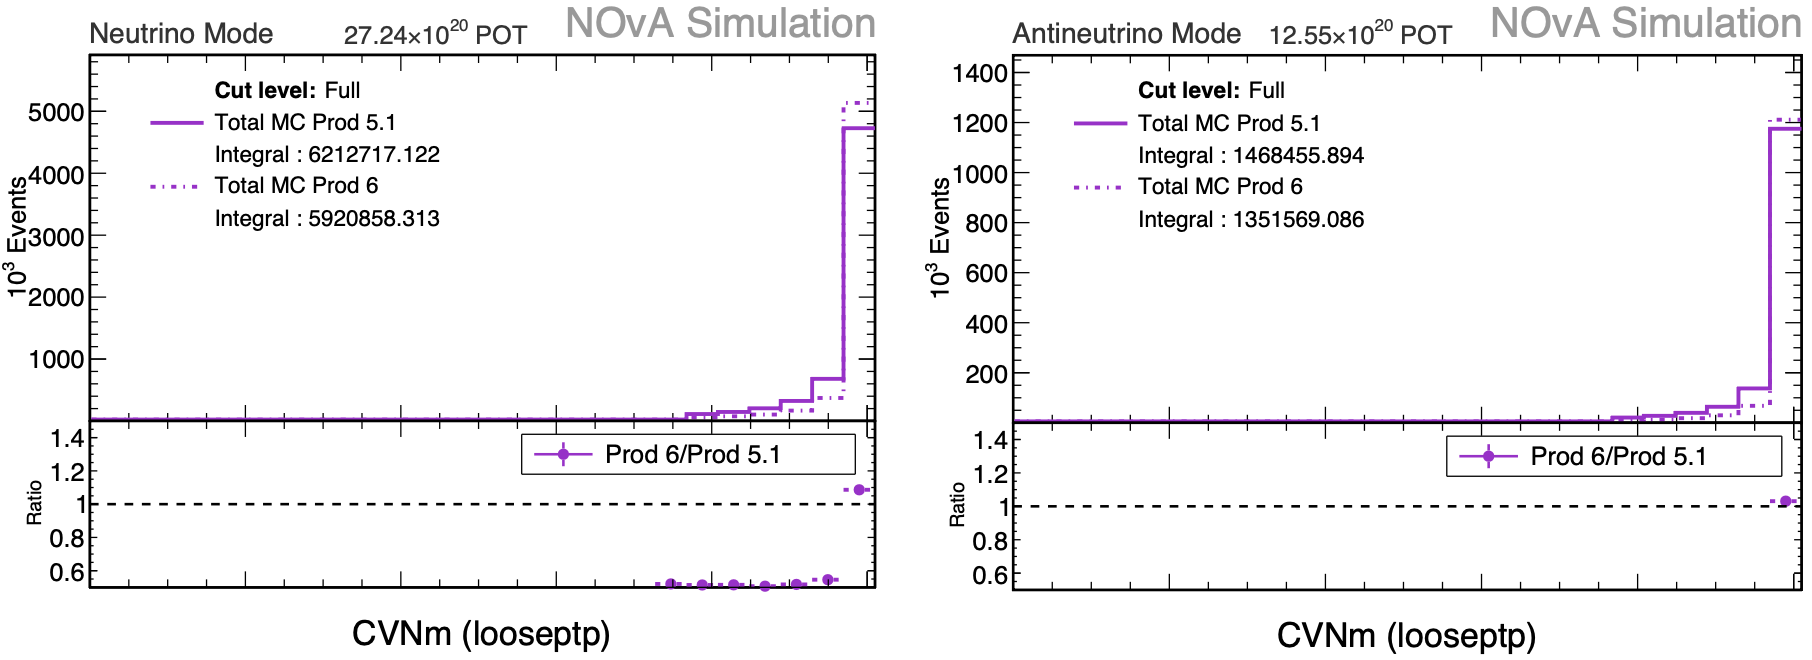
\includegraphics[width=1\textwidth]{images-ochow/nd-cvn-first-talk.png}%
    }{%
        \fbox{\parbox[c][0.2\textheight][c]{0.65\textwidth}{\centering Placeholder: \texttt{images-ochow/nd-cvn-first-talk.png}}}%
    }
    \caption{ND $\nu_{\mu}$ CVN classifier score after the full Ana2024 selection for FHC (left) and RHC (right), comparing Prod~6 (transformerCVN) and Prod~5.1~\cite{ochow-nd-numu-init}.
    The Prod~6 distribution is more peaked towards 1, indicating improved PID performance.}
    \label{fig:nd-cvn-first-talk}
\end{figure}

The second talk \cite{ochow-nd-numu-mctomc} builds on the first one by investigating the effect of the cutflow on each sample, using the efficiency w.r.t.\ no cut and purity defined in App.~\ref{app:cutflow}.

This is followed by looking more closely at the CVN variable in both productions, including a breakdown into its signal and background components.
This motivates the need to retune the PID cut values for the Prod~6 CVN.

The third talk \cite{ochow-nd-numu-cvn} begins in a similar way, but acknowledges an oversight in the previous two talks, that is, for the Prod~5.1 distributions, the Genie skew fix and chase weights were not applied.
This was corrected in the third talk, with this change being carried over to the rest of the comparisons.
The talk also defines a new signal definition as $\nu_\mu/\bar\nu_\mu$ CC inside a fiducial volume defined based on the shower start and stop boundaries and Kalman track start requirements in \texttt{kNumuContainND2024}.
The $\nu_\mu$ classification score variable was once again investigated more closely, by breaking the distribution down into its signal and background components.
TransformerCVN was found to be more peaked in each components except for $\nu_e/\bar\nu_e$, indicating an overall better performance.
The talk also goes through an efficiency-matching procedure to retune the PID cut values in Prod~6 for the transformerCVN cut, based on the Prod~5.1 CVN cut (\texttt{kCVNm\_looseptp}) at 0.76.
This was done by finding the transformerCVN cut value in Prod~6 that gave a signal efficiency that matched the Prod~5.1 signal efficiency after quality, containment and the CVN cut value were applied.
This is shown in Fig.~\ref{fig:nd-numu-cvn-eff-match}.

\begin{figure}[htbp]
    \centering
    \IfFileExists{images-ochow/nd-numu-eff-match.png}{%
        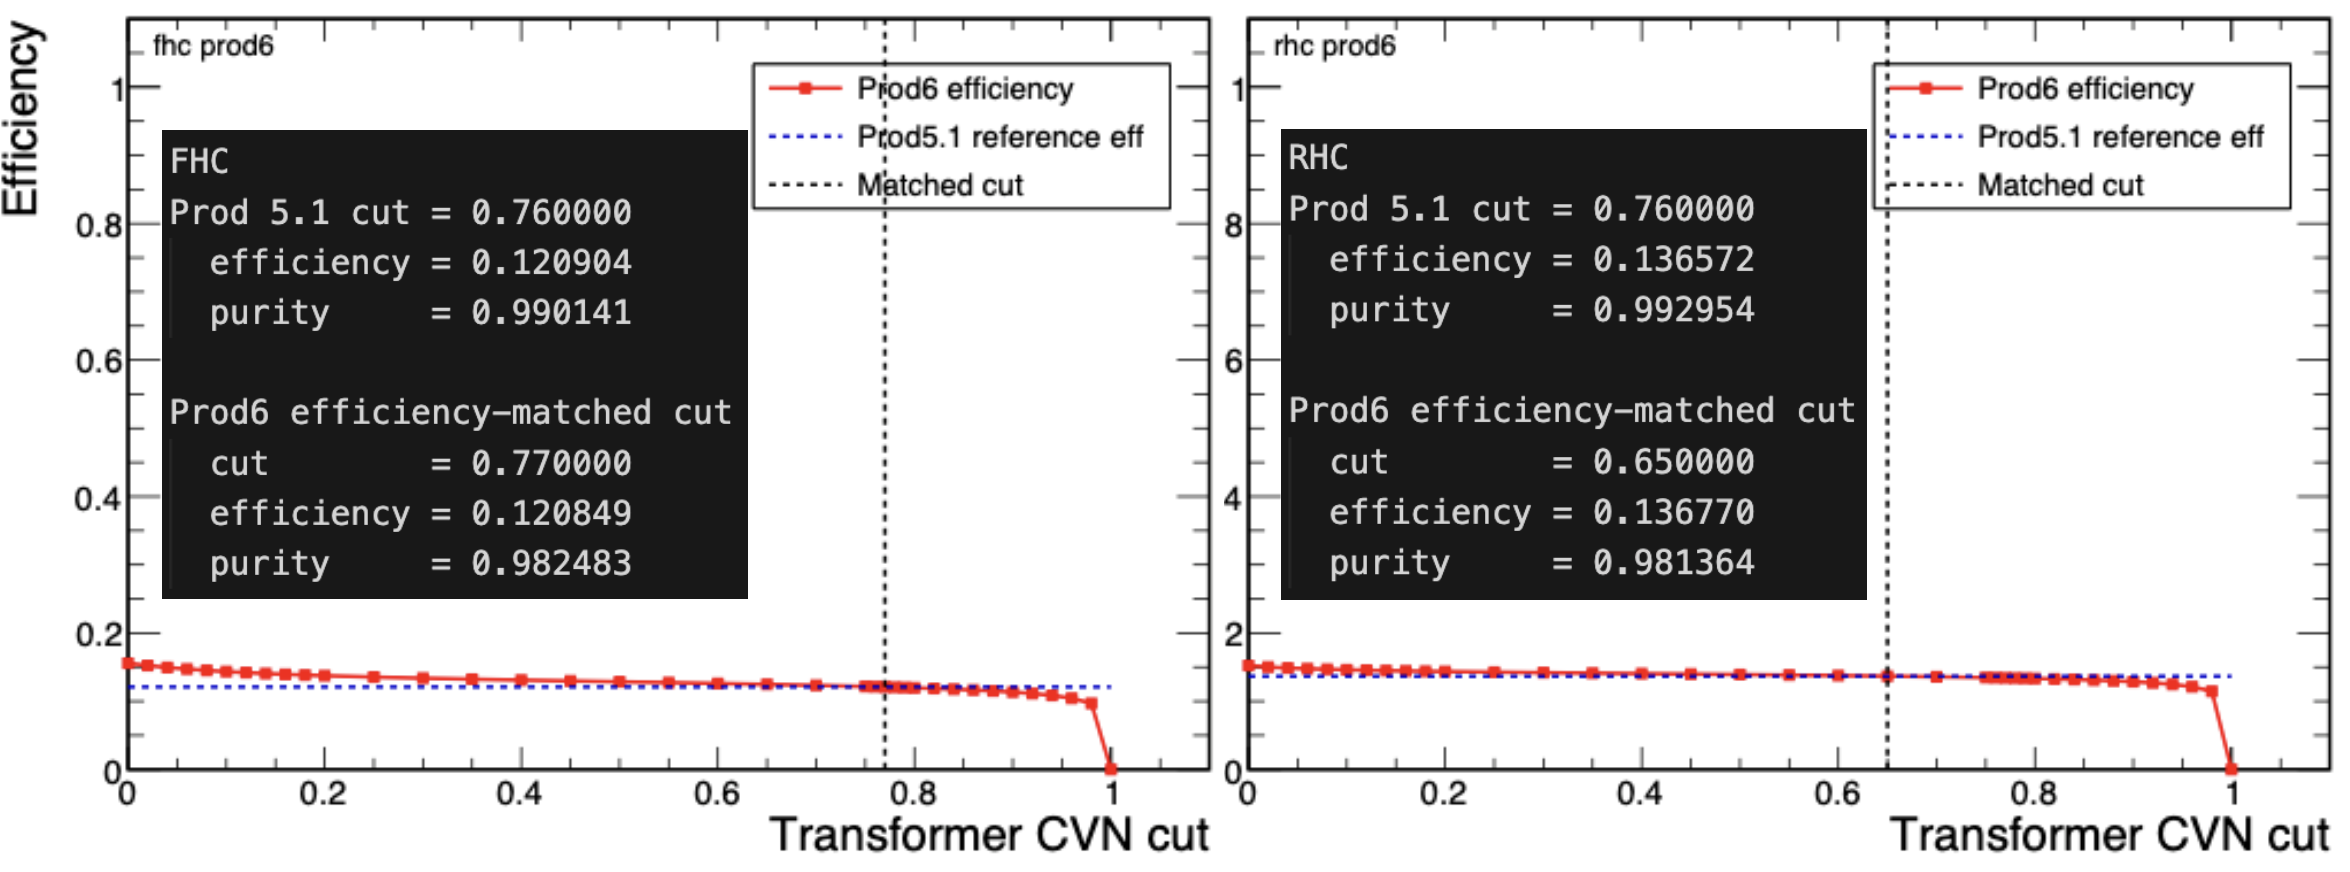
\includegraphics[width=1\textwidth]{images-ochow/nd-numu-eff-match.png}%
    }{%
        \fbox{\parbox[c][0.2\textheight][c]{0.65\textwidth}{\centering Placeholder: \texttt{images-ochow/nd-numu-eff-match.png}}}%
    }
    \caption{Efficiency-matched TransformerCVN threshold for Prod~6: Prod~6 selection efficiency vs.\ TransformerCVN cut (red) matched to the Prod~5.1 reference efficiency (blue dashed) at the 0.76 cut value , yielding retuned thresholds of 0.77 (FHC) and 0.65 (RHC)~\cite{ochow-nd-numu-cvn}.}
    \label{fig:nd-numu-cvn-eff-match}
\end{figure}

\subsection{FD: \texorpdfstring{$\nu_\mu$}{numu} MC to MC Comparisons \& efficiency studies}
My work on the FD $\nu_{\mu}$ side was captured in one talk~\cite{ochow-fd-numu-sel}.
In addition to the Prod~5.1 and Prod~6 files, this talk also considered the so-called rereco sample \footnote {This sample is produced by running the Prod~5.1 reconstruction chain on the Prod~6 simulation.}.
The comparisons done in this talk were performed in a similar fashion to the ND $\nu_{\mu}$ side.
Comparisons of variable distributions at each cutflow stage including the full selection were done in both horn currents.
These were accompanied by efficiencies, defined in Apps.~\ref{app:cutflow} and~\ref{app:sequential}, which were computed at each cutflow stage, and tabulated.

The cutflow tables in the talk show that the sequential and total signal efficiencies are very similar across all three samples after the full FD selection.
Table~\ref{tab:fd-numu-cutflow-rhc} shows the RHC cutflow summary comparing the three samples.
Comparing Prod~6 with the rereco sample isolates the effect of the reconstruction on the same Prod~6 simulation.
The Prod~6 reconstruction gives a slightly higher signal efficiency with respect to the no-cut level (0.145 vs.\ 0.142), but a slightly lower purity (97.8\% vs.\ 98.4\%).
This is already achieved without a full re-optimisation of any PID or quantile cuts in Prod~6, suggesting that the reconstruction changes alone give a comparable performance with a small differences in the efficiency--purity. 
Full reoptimisation of these cuts in Prod~6 may yield better results.
Finally, $n$-1 efficiencies (App.~\ref{app:nminus1}) were calculated to isolate the cosmic rejection cut~\cite{ochow-fd-numu-sel}.
\begin{table}[htbp]
    \centering
    \caption{FD $\nu_\mu$ cutflow summary at the full selection in RHC for Prod~5.1, Prod~6, and the rereco sample~\cite{ochow-fd-numu-sel}.
    The rereco and Prod~6 samples share the same Prod~6 simulation and differ only in reconstruction; rereco and Prod~5.1 share the same reconstruction and differ only in simulation.}
    \label{tab:fd-numu-cutflow-rhc}
    \vspace{0.9em}
    \begin{tabular}{lccccc}
        \hline
        Sample & Reco & Sim & Signal eff.\ (w.r.t.\ no cut) & Purity (\%) \\
        \hline
        Prod~5.1  & 5.1 & 5.1 & 0.156 & 98.4 \\
        rereco    & 5.1 & 6   & 0.142 & 98.4 \\
        Prod~6    & 6   & 6   & 0.145 & 97.8 \\
        \hline
    \end{tabular}
\end{table}

A key result of this study is illustrated in Fig.~\ref{fig:ochow-fd-numu-rereco}, which shows the $\nu_\mu$ energy distribution at the FD after the full selection, oscillated about the Asimov $Z$ point.
The Prod~6 and rereco samples, which differ only in their reconstruction, are in close agreement, with small differences visible in the ratio plot.
In contrast, despite sharing the same reconstruction chain as the rereco sample, the Prod~5.1 distribution sits higher than both other samples.
Since these samples only differ in the underlying simulation, this indicates that the shift in the distribution from Prod~5.1 to Prod~6 is mostly driven by these simulation changes rather than in the reconstruction. These findings are consistent with expectations from other studies~\cite{tricia-xsec-prod6}.
This behaviour is consistent throughout other variables as well as in both horn currents.

\begin{figure}[htbp]
    \centering
    \begin{minipage}[t]{0.48\textwidth}
        \centering
        \IfFileExists{images-ochow/fd-numu-rereco.png}{%
            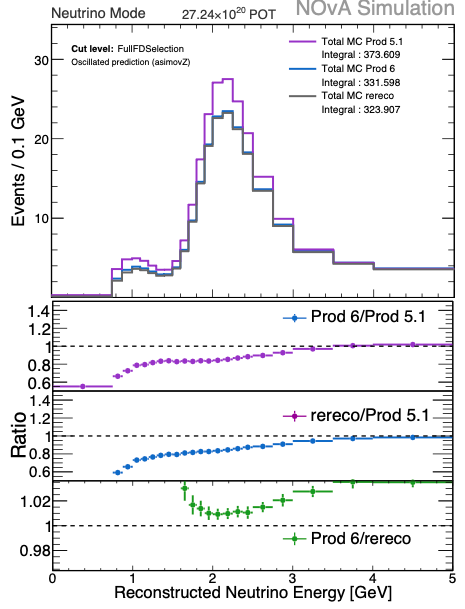
\includegraphics[width=\textwidth]{images-ochow/fd-numu-rereco.png}%
        }{%
            \fbox{\parbox[c][0.18\textheight][c]{\textwidth}{\centering Placeholder: \texttt{fd-numu-rereco.png}}}%
        }
    \end{minipage}
    \hfill
    \begin{minipage}[t]{0.48\textwidth}
        \centering
        \IfFileExists{images-ochow/fd-numu-rereco-rhc.png}{%
            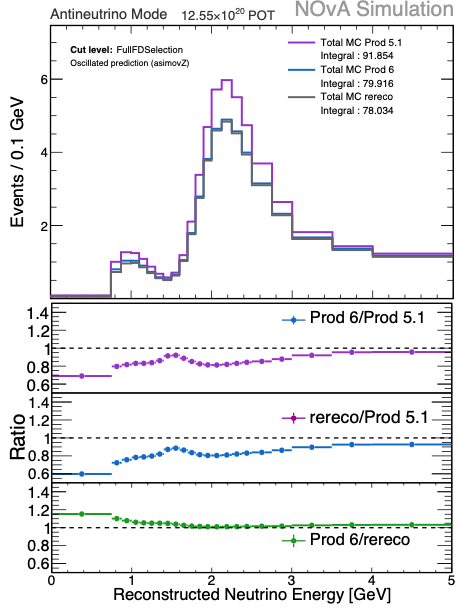
\includegraphics[width=\textwidth]{images-ochow/fd-numu-rereco-rhc.png}%
        }{%
            \fbox{\parbox[c][0.18\textheight][c]{\textwidth}{\centering Placeholder: \texttt{fd-numu-rereco-rhc.png}}}%
        }
    \end{minipage}
    \caption{FD $\nu_\mu$ energy distribution after the full selection, oscillated about the Asimov~$Z$ point, for FHC (left) and RHC (right)~\cite{ochow-fd-numu-sel}.
    In both horn currents the Prod~6 and rereco samples, which differ only in reconstruction, are in close agreement.
    The higher Prod~5.1 distribution, which shares the same reconstruction as rereco, suggests the observed shift is primarily due to simulation rather than reconstruction changes.}
    \label{fig:ochow-fd-numu-rereco}
\end{figure}

\subsection{FD: \texorpdfstring{$\nu_e$}{nue} MC to MC Comparisons}
My work on the FD $\nu_e$ side was captured in two talks~\cite{ochow-fd-nue-vtx,ochow-fd-nue-2}.
~\cite{ochow-fd-nue-vtx} shows initial $\nu_e$ comparisons with similar analysis details as those used in the previous talks.
The distributions were separated in the three subsamples of the FD $\nu_e$ analysis binning.
They show large differences between the three distributions (Fig.~\ref{fig:ochow-fd-nue-retune}, left plot showing CVNe Low bin of the core sample).
This is due to the PID cuts used for all samples were the ones optimised for the Prod~5.1 analysis.
The cuts needed retuning in Prod~6 for reliable comparisons.
The retuning of all of the $\nu_e$ PID cuts was done by Hanyi Chen via efficiency matching, in a similar fashion to the ND $\nu_{\mu}$ side.
~\cite{ochow-fd-nue-2} shows the follow up after this retuning.
It was also asked to breakdown each $\nu_e$ analysis bin subsample into its constituent  signal and background components.
Following the retuning, the three production distributions agree more closely (Fig.~\ref{fig:ochow-fd-nue-retune}, right).
This agreement is consistent throughout other variables.

\begin{figure}[htbp]
    \centering
    \begin{minipage}[t]{0.48\textwidth}
        \centering
        \IfFileExists{images-ochow/fd-nue-before-retune.png}{%
            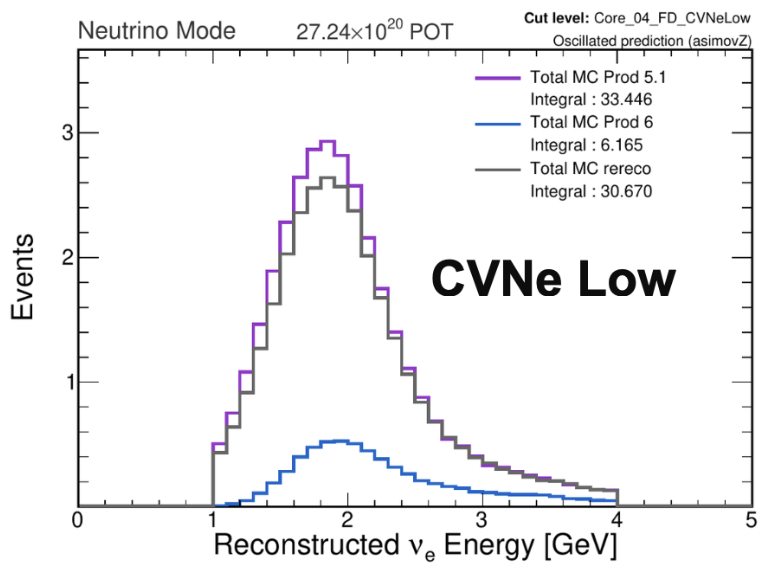
\includegraphics[width=\textwidth]{images-ochow/fd-nue-before-retune.png}%
        }{%
            \fbox{\parbox[c][0.18\textheight][c]{\textwidth}{\centering Placeholder: \texttt{fd-nue-before-retune.png}}}%
        }
    \end{minipage}
    \hfill
    \begin{minipage}[t]{0.48\textwidth}
        \centering
        \IfFileExists{images-ochow/fd-nue-after-retune.png}{%
            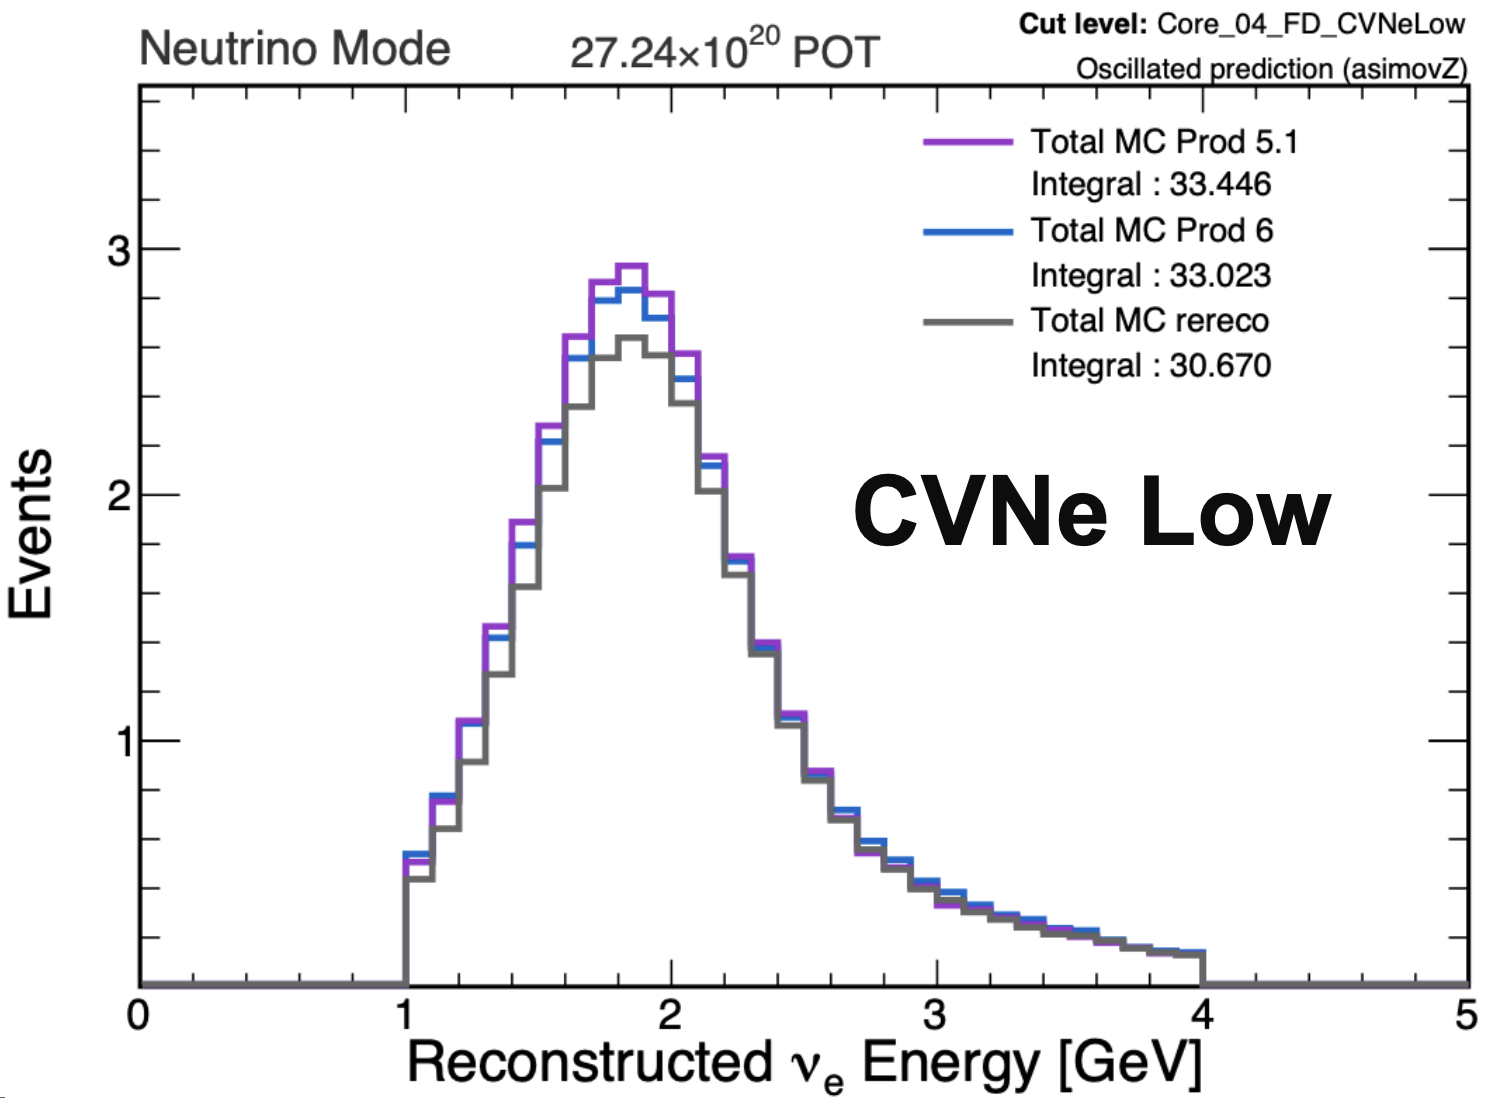
\includegraphics[width=\textwidth]{images-ochow/fd-nue-after-retune.png}%
        }{%
            \fbox{\parbox[c][0.18\textheight][c]{\textwidth}{\centering Placeholder: \texttt{fd-nue-after-retune.png}}}%
        }
    \end{minipage}
    \caption{Representative FD $\nu_e$ selection variable in FHC before (left) and after (right) PID retuning~\cite{ochow-fd-nue-vtx,ochow-fd-nue-2}.}
    \label{fig:ochow-fd-nue-retune}
\end{figure}

\subsection{FD: Vertex-Finding Failures in Prod~6}

There were some reports of vertex-finding failures in Prod~6, so an efficiency study was carried out.
The first part of the study belongs in the second half of~\cite{ochow-fd-nue-vtx}.
Vertex-finding efficiency (App.~\ref{app:vtx-eff}) was computed bin-by-bin to investigate where these failures were occurring.

Comparing Prod~6 with Prod~5.1, the vertex variables showed that the vertex-finding efficiency dropped at the edges of the detectors.
To understand why, the slice NHits variable was considered.
Fig.~\ref{fig:fd-vtx-nhits} shows that Prod~6 does not return a valid vertex below 15 hits, consistent with the \texttt{mlvertex} implementation.
Above 15 hits, Prod~6 reaches 100\% vertex-finding efficiency, whereas Prod~5.1 turns on gradually and only approaches 100\% around $25$ hits.
The efficiency drops at the edges of the detector as shown by the true vertex position variables are likely related to events that are partially contained and therefore have fewer recorded hits.

\begin{figure}[htbp]
    \centering
    \begin{minipage}[t]{0.48\textwidth}
        \centering
        \IfFileExists{images-ochow/nhit_zoom_nue_eff_overlay.pdf}{%
            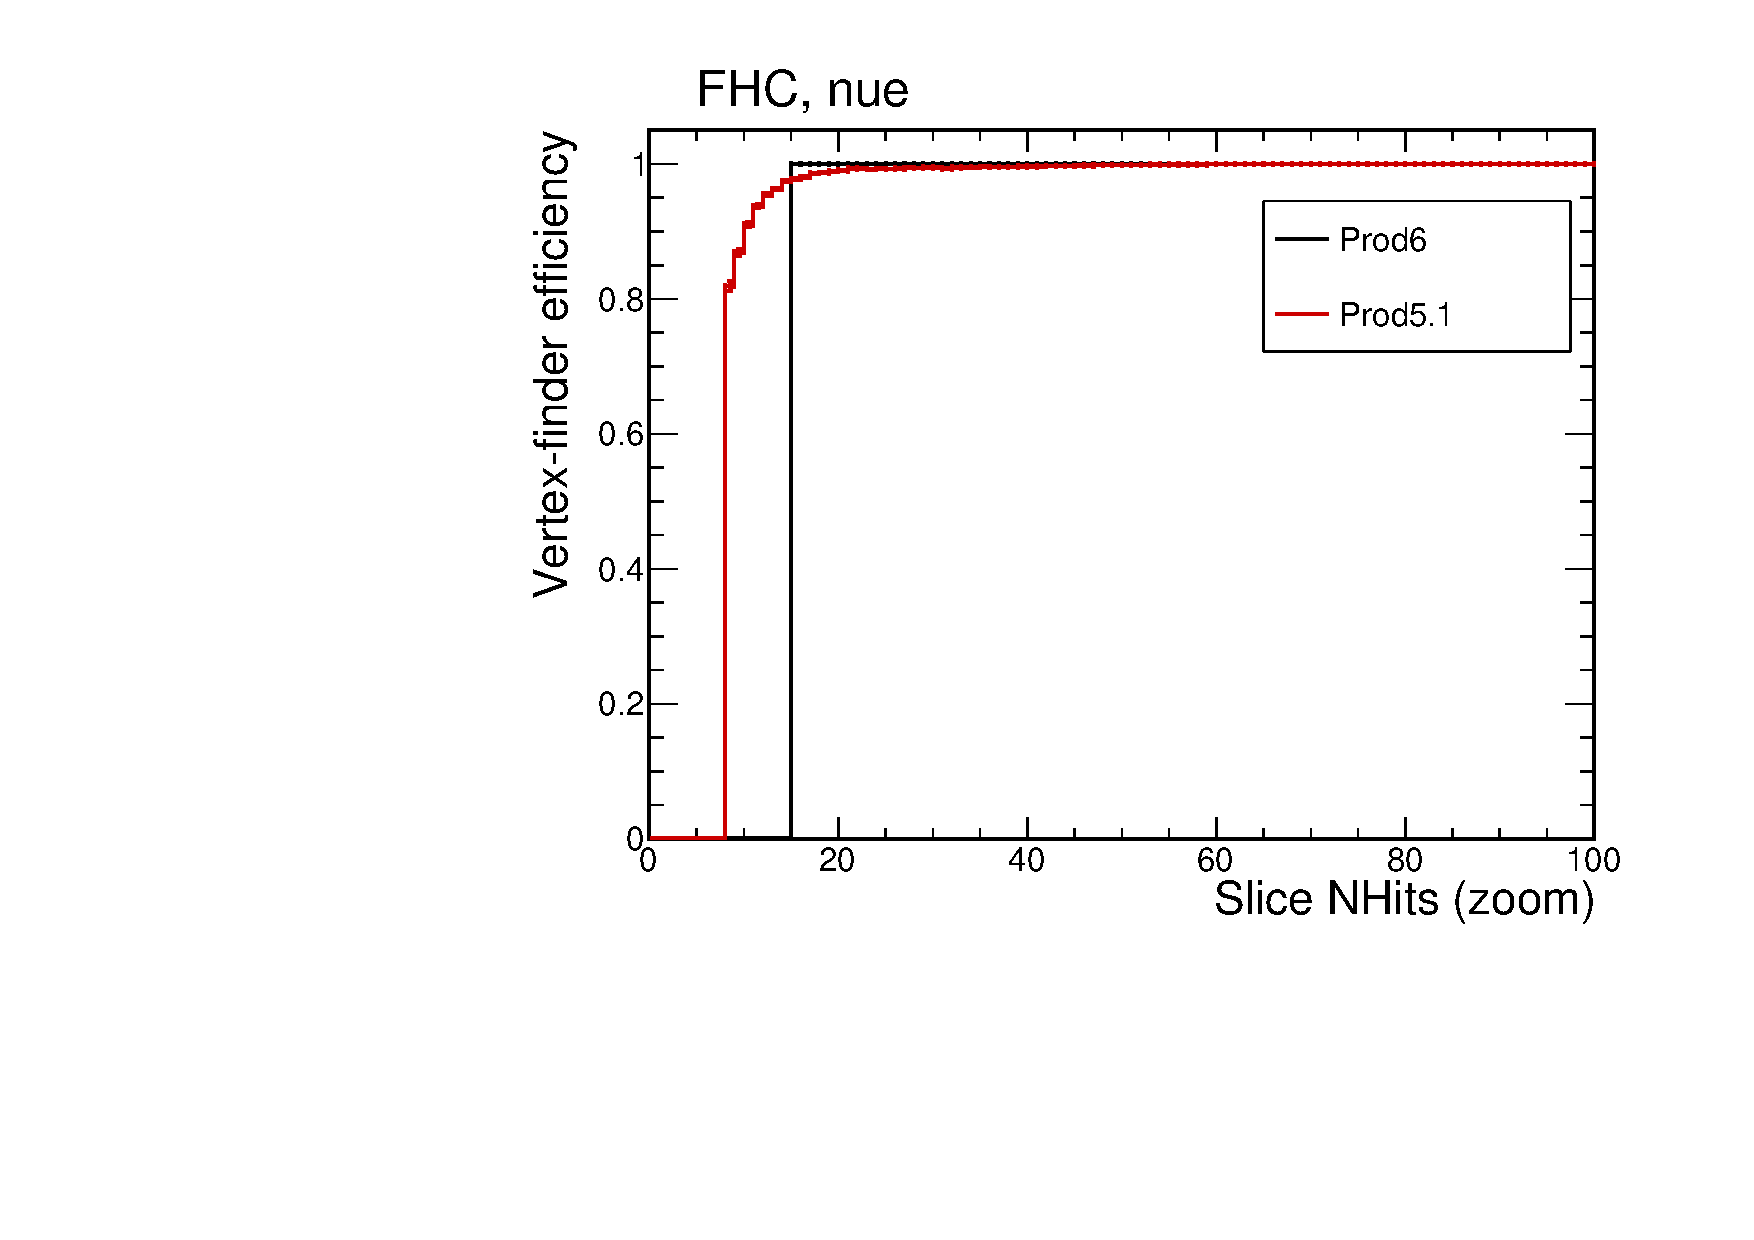
\includegraphics[width=\textwidth]{images-ochow/nhit_zoom_nue_eff_overlay.pdf}%
        }{%
            \fbox{\parbox[c][0.18\textheight][c]{\textwidth}{\centering Placeholder: \texttt{nhit\_zoom\_nue\_eff\_overlay.pdf}}}%
        }
    \end{minipage}
    \hfill
    \begin{minipage}[t]{0.48\textwidth}
        \centering
        \IfFileExists{images-ochow/nhit_zoom_numu_eff_overlay.pdf}{%
            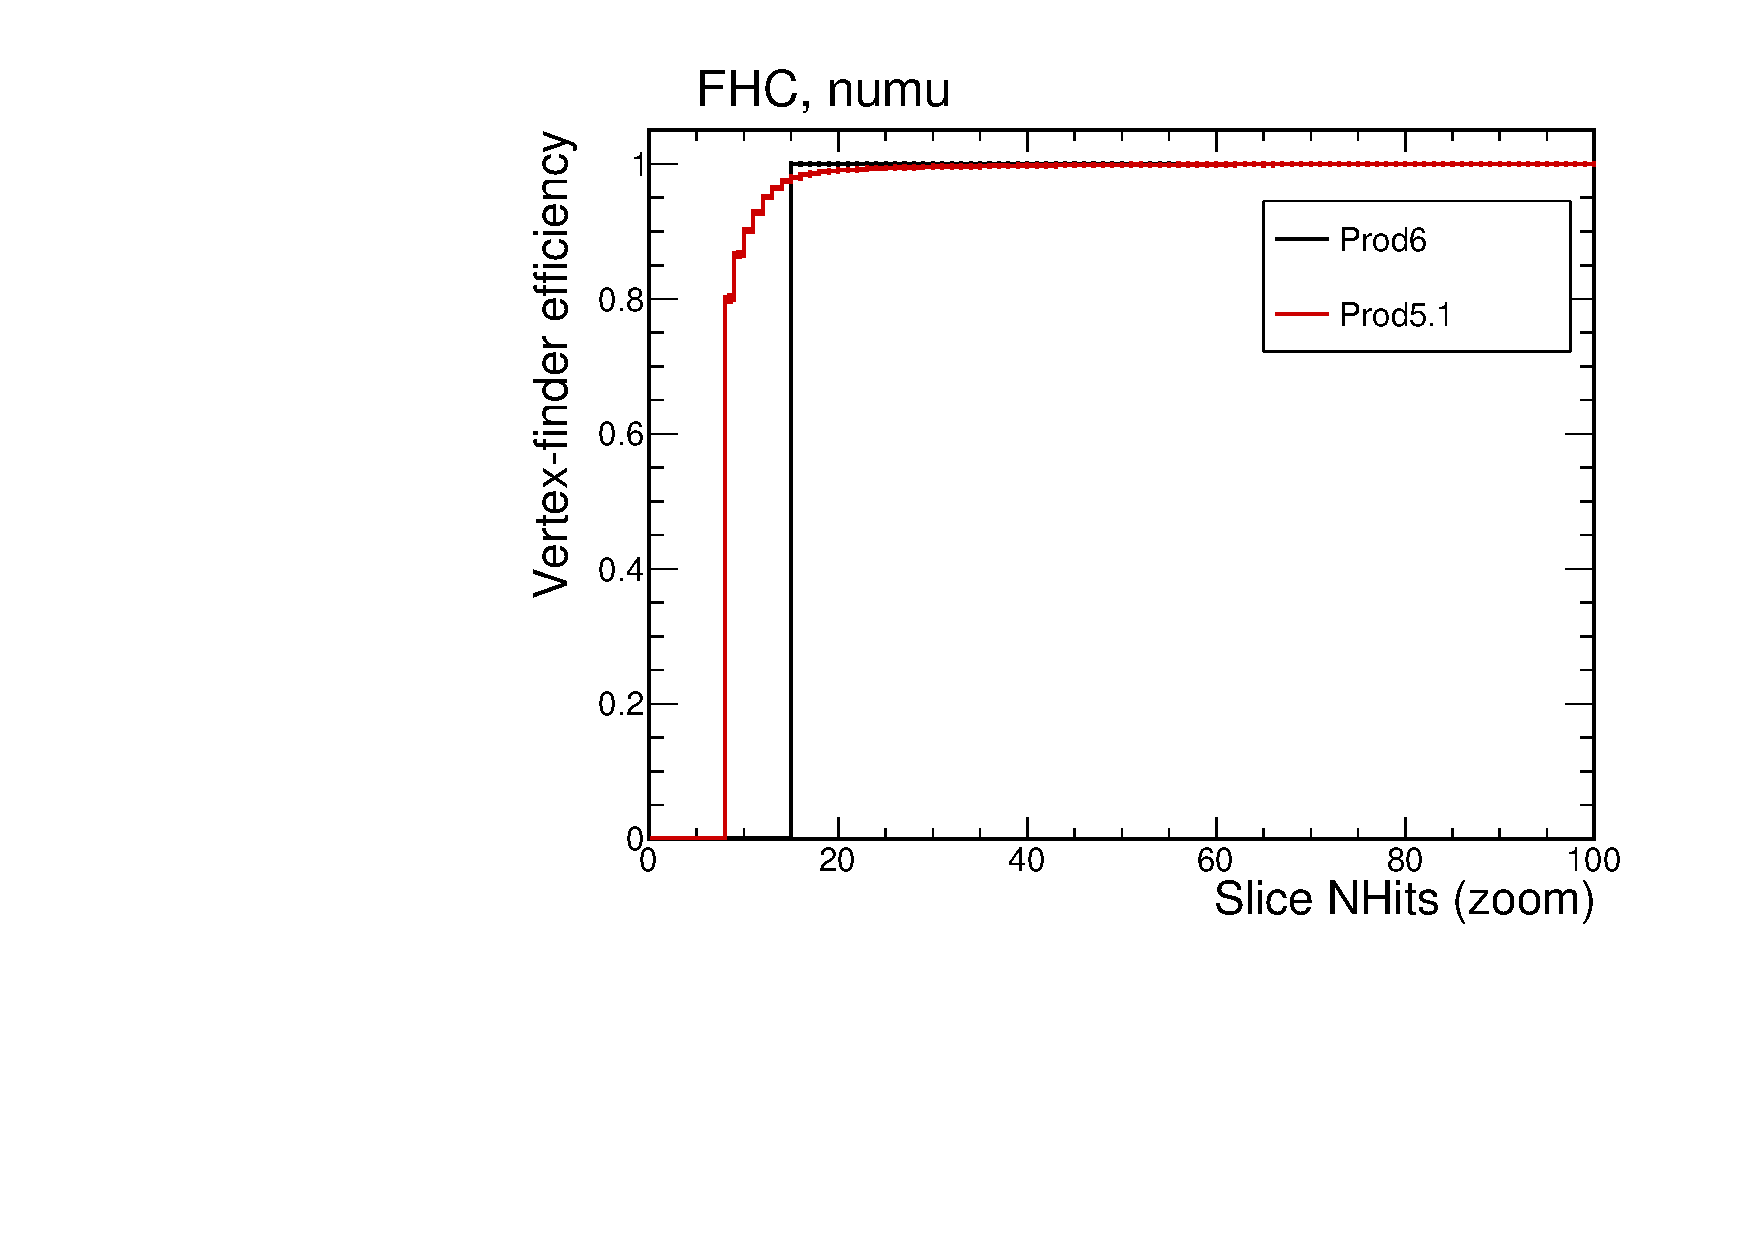
\includegraphics[width=\textwidth]{images-ochow/nhit_zoom_numu_eff_overlay.pdf}%
        }{%
            \fbox{\parbox[c][0.18\textheight][c]{\textwidth}{\centering Placeholder: \texttt{nhit\_zoom\_numu\_eff\_overlay.pdf}}}%
        }
    \end{minipage}
    \caption{Vertex-finding efficiency vs.\ slice NHits (zoomed, 0--30 range) for FHC $\nu_e$ signal (left) and $\nu_\mu$ CC (right), comparing Prod~6 and Prod~5.1 without any NHits selection applied~\cite{ochow-fd-nue-vtx}.
    Prod~6 does not return a valid vertex below 15 hits, consistent with the \texttt{mlvertex} pixel-map requirement, and reaches 100\% efficiency above this threshold.
    Prod~5.1 turns on gradually, approaching 100\% only around $25$ hits.}
    \label{fig:fd-vtx-nhits}
\end{figure}

To address some requests, ~\cite{ochow-fd-vertex-2} was conducted.
One such request was to apply the basic quality NHits requirements used in the FD selections (30 hits for $\nu_e$, 20 for $\nu_\mu$, a cut on 30 hits was used for throughout).
The effect of this cut was that in Prod~6, the vertex-finding efficiency was found do be almost 100\% across the detector (Fig.~\ref{fig:ochow-fd-vtx-x}).
This cut also removes the lower vertex-finding efficiency at low true neutrino energies exhibited before this nhits cut on all production sample.

\begin{figure}[htbp]
    \centering
    \begin{minipage}[t]{0.48\textwidth}
        \centering
        \IfFileExists{images-ochow/vtx_x_nue_eff_overlay_zoom.pdf}{%
            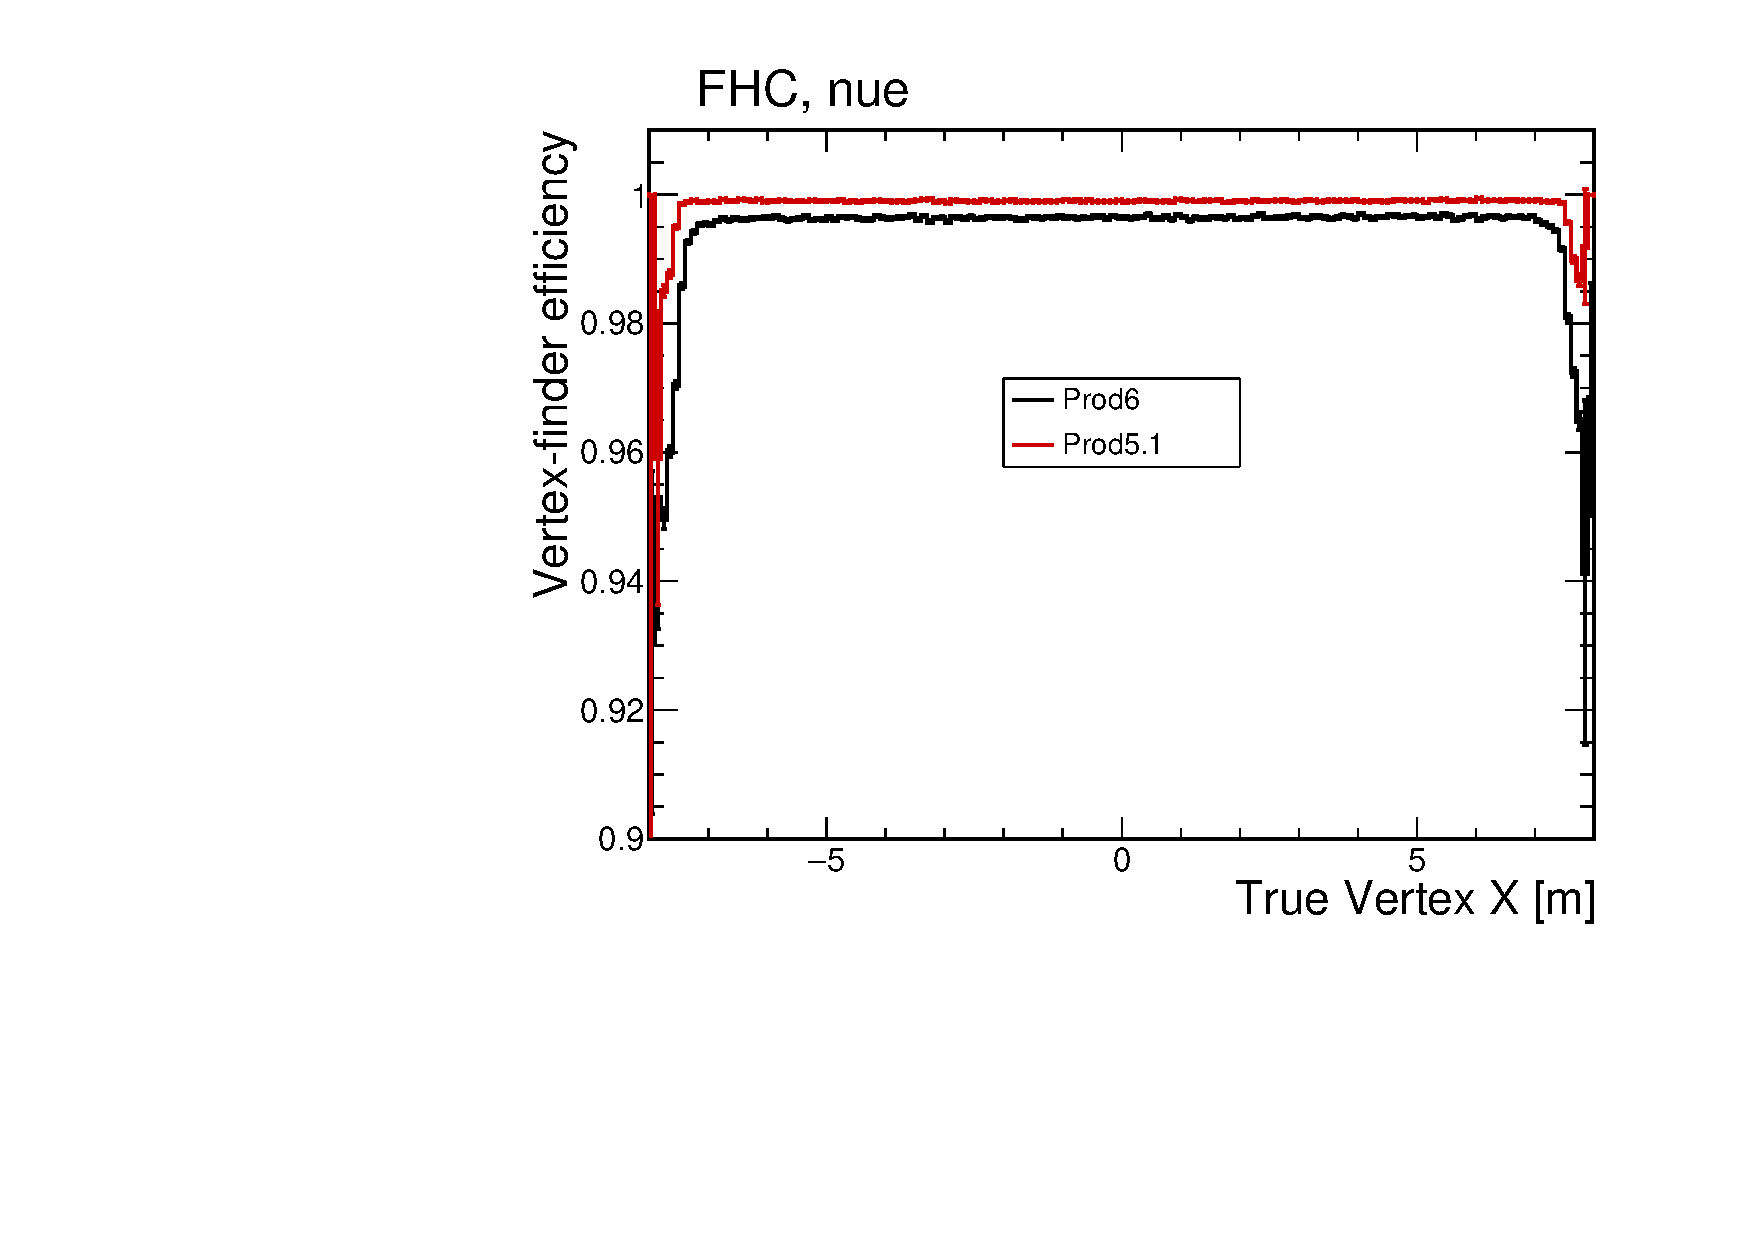
\includegraphics[width=\textwidth]{images-ochow/vtx_x_nue_eff_overlay_zoom.pdf}%
        }{%
            \fbox{\parbox[c][0.18\textheight][c]{\textwidth}{\centering Placeholder: \texttt{vtx\_x\_nue\_eff\_overlay\_zoom.pdf}}}%
        }
    \end{minipage}
    \hfill
    \begin{minipage}[t]{0.48\textwidth}
        \centering
        \IfFileExists{images-ochow/vtx_x_numu_eff_overlay_zoom.pdf}{%
            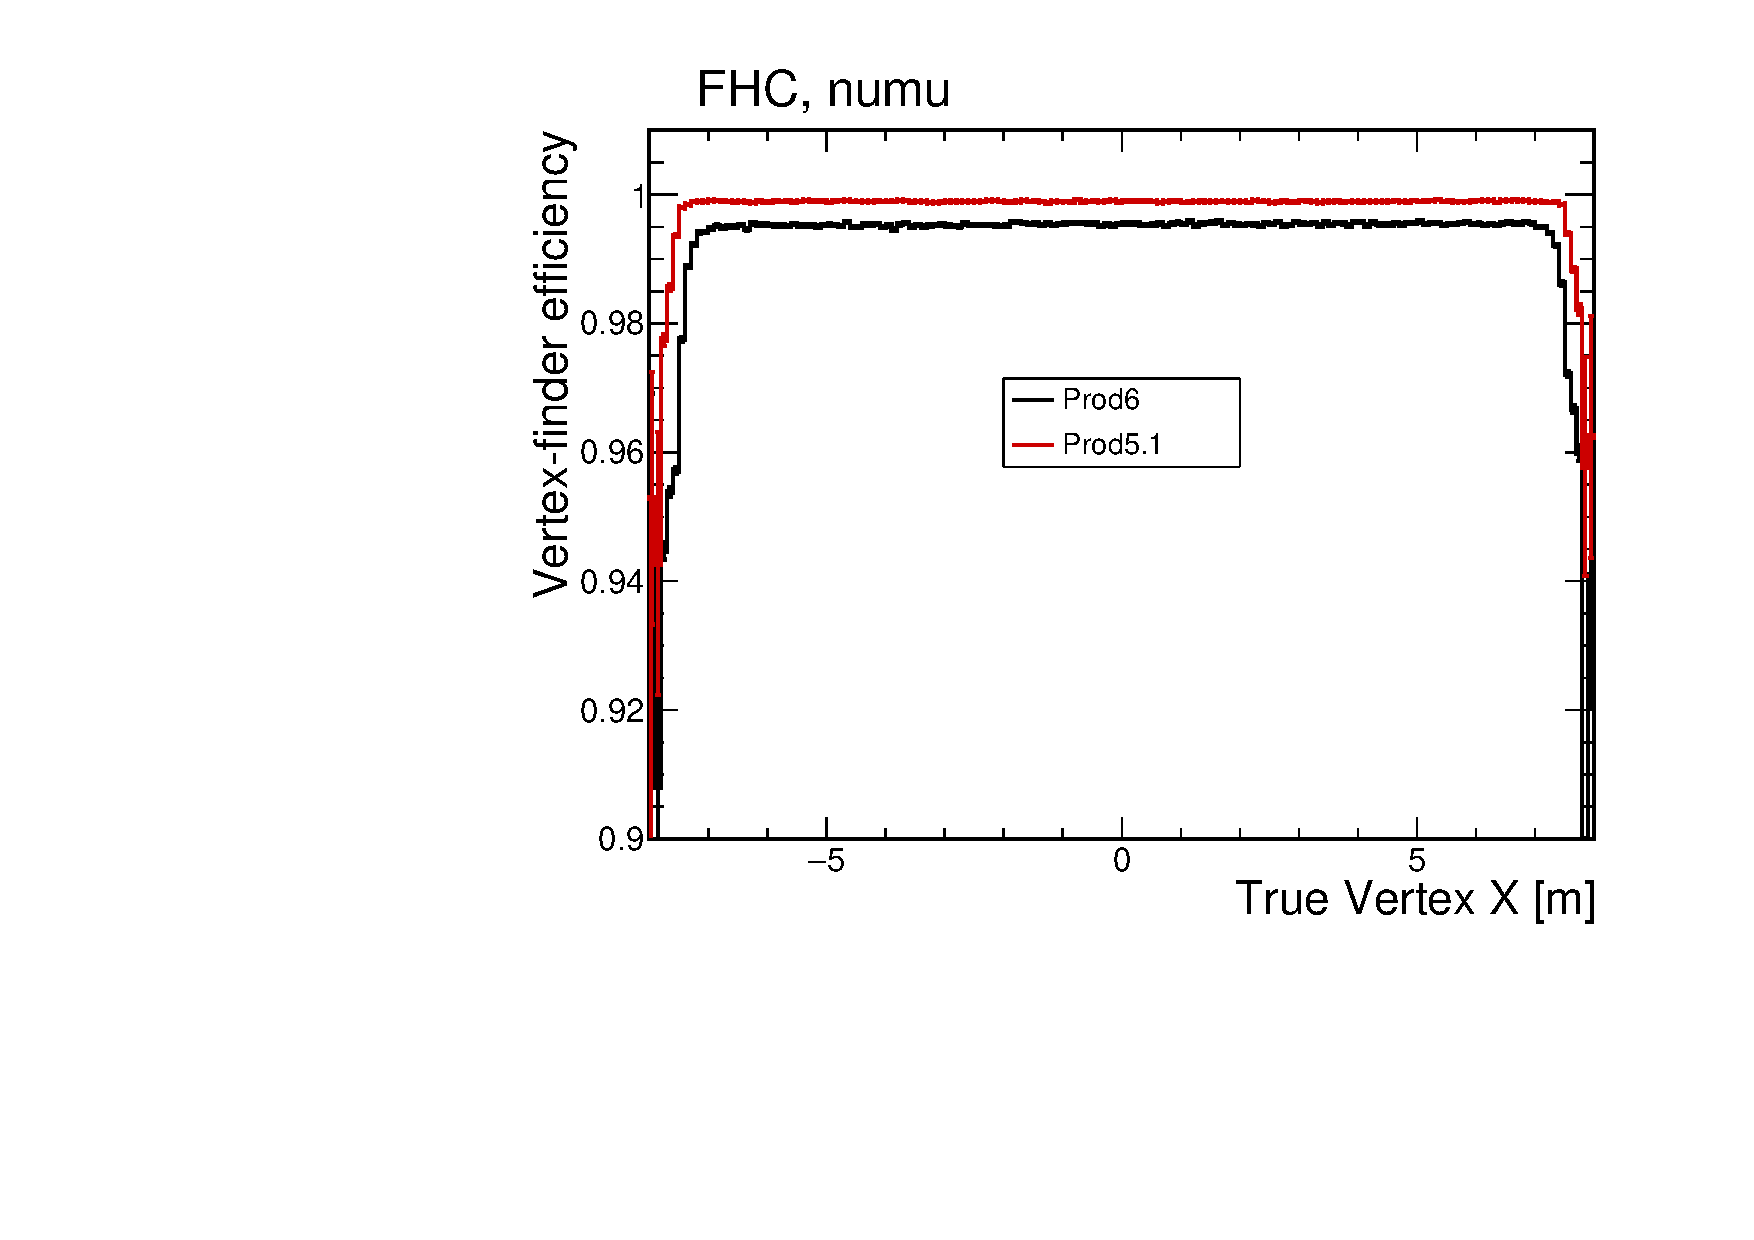
\includegraphics[width=\textwidth]{images-ochow/vtx_x_numu_eff_overlay_zoom.pdf}%
        }{%
            \fbox{\parbox[c][0.18\textheight][c]{\textwidth}{\centering Placeholder: \texttt{vtx\_x\_numu\_eff\_overlay\_zoom.pdf}}}%
        }
    \end{minipage}
    \caption{Vertex-finding efficiency vs.\ true vertex $x$ position (FHC) for $\nu_e$ signal (left) and $\nu_\mu$ CC (right) after applying NHits $> 30$, comparing Prod~6, Prod~5.1, and rereco~\cite{ochow-fd-vertex-2}.
    Prod~6 (\texttt{mlvertex}) achieves $\approx 100\%$ efficiency throughout the detector; Prod~5.1 and rereco still show some residual failures.}
    \label{fig:ochow-fd-vtx-x}
\end{figure}

In Prod~6, vertex-finding failures are always associated with failure to produce a valid CVN map (App.~\ref{app:cvn-vtx-eff}; \texttt{rec.training.cvnmapsfilled}$=1$).
A valid CVN map always yields a valid vertex, something that does not hold in Prod~5.1.
Vertex resolution plots for events with valid vertices was shown to be tighter and more peaked in Prod~6 compared to Prod~5.1 and rereco (Fig.~\ref{fig:ochow-fd-vtx-res}).

\begin{figure}[htbp]
    \centering
    \IfFileExists{images-ochow/fd-vtx-res.png}{%
        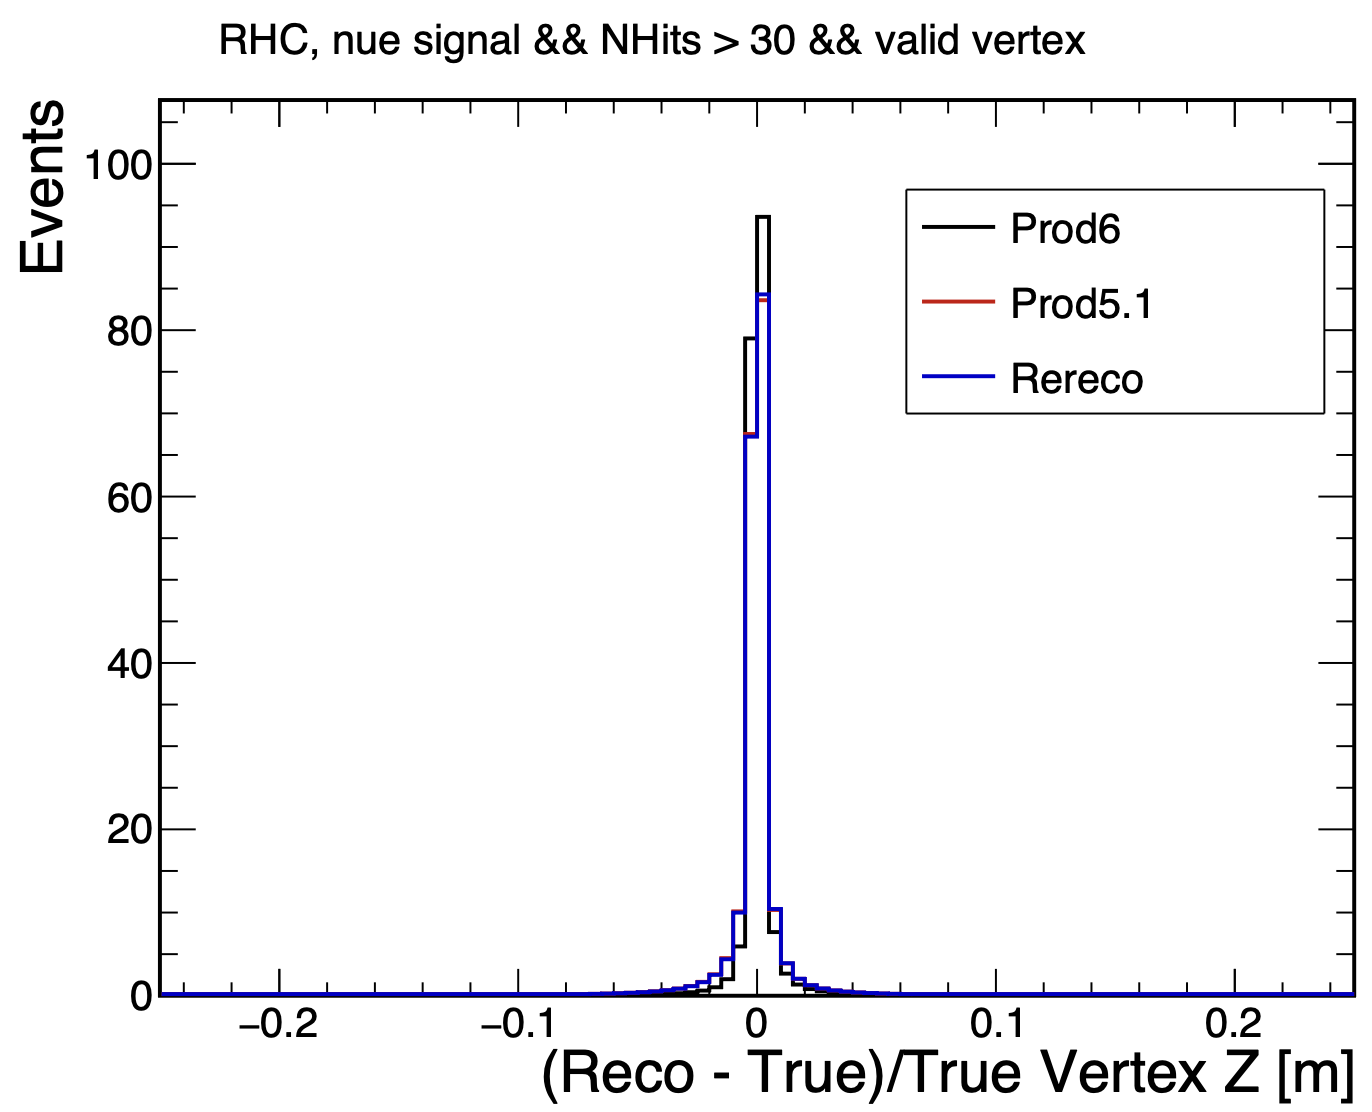
\includegraphics[width=0.65\textwidth]{images-ochow/fd-vtx-res.png}%
    }{%
        \fbox{\parbox[c][0.2\textheight][c]{0.65\textwidth}{\centering Placeholder: \texttt{images-ochow/fd-vtx-res.png}}}%
    }
    \caption{$(\mathrm{Reco}-\mathrm{True})/\mathrm{True}$ vertex $z$ for RHC $\nu_e$ signal with NHits $> 30$ and valid vertex, comparing Prod~6, Prod~5.1, and rereco~\cite{ochow-fd-vertex-2}.}
    \label{fig:ochow-fd-vtx-res}
\end{figure}

The talk also highlights a brief check for peripheral $\nu_e$ and NuX NC samples, which do not have an explicit NHits cut.
It was verified that no Prod~5.1 events with fewer than 15 hits pass the final selection for these samples, confirming the mlvertex 15-hit requirement does not affect existing selections.

\appendix
\section{Efficiency and purity definitions}
\label{app:eff-defs}

The quantities below are used in the ND and FD $\nu_{\mu}$ cutflow studies and the FD vertex-finding studies summarised above.

\subsection{Cutflow quantities}
\label{app:cutflow}

At each stage $i$ of the selection cutflow:
\begin{itemize}
    \item \textbf{Total selected events} --- the number of events passing all cuts applied up to level~$i$ (signal plus background).
    \item \textbf{True $\nu_{\mu}$ CC efficiency} (w.r.t.\ no cut) --- fraction of signal surviving cut level~$i$ relative to \texttt{kNoCut}:
    \begin{equation}
        \varepsilon_{\nu_{\mu}\mathrm{CC}}[i] = \frac{N_\mathrm{sig}^\mathrm{cut}[i]}{N_\mathrm{sig}^\mathrm{cut}[\mathrm{NoCut}]}\,.
        \label{eq:cutflow-eff-nocut}
    \end{equation}
    \item \textbf{Purity} --- fraction of selected events that are true signal:
    \begin{equation}
        \mathrm{Purity} = \frac{N_\mathrm{true}(\mathrm{sig})}{N_\mathrm{selected}(\mathrm{total})}\,.
        \label{eq:purity}
    \end{equation}
\end{itemize}

\subsection{Sequential efficiency}
\label{app:sequential}

Efficiency at cut level~$i$ relative to the previous cut level:
\begin{equation}
    \varepsilon_{\nu_{\mu}\mathrm{CC}}^\mathrm{seq}[i] = \frac{N_\mathrm{sig}^\mathrm{cut}[\mathrm{level}_i]}{N_\mathrm{sig}^\mathrm{cut}[\mathrm{level}_{i-1}]}\,.
    \label{eq:sequential-eff}
\end{equation}
\noindent Isolates the effect of each cut when applied in sequence.

\subsection{$n$-1 efficiency}
\label{app:nminus1}

Efficiency with all cuts applied except cut~$i$:
\begin{equation}
    \varepsilon_{n-1}[i] = \frac{N_\mathrm{sig}^\mathrm{cut}[\mathrm{all}]}{N_\mathrm{sig}^\mathrm{cut}[\mathrm{all}-i]}\,.
    \label{eq:nminus1-eff}
\end{equation}
\noindent Measures the effect of a single cut with all others already applied.

\subsection{Vertex-finding efficiency}
\label{app:vtx-eff}

Computed bin-by-bin for $\nu_e$ signal (\texttt{kIsSig}) and $\nu_{\mu}$ CC signal (\texttt{kIsNumuCC}), with no other cuts applied:
\begin{equation}
    \varepsilon_i = \frac{N_\mathrm{num}(x_i)}{N_\mathrm{den}(x_i)}\,,
    \label{eq:vtx-eff}
\end{equation}
where $N_\mathrm{num}$ counts signal events with \texttt{vtx.mlvertex.IsValid}$=1$ and $N_\mathrm{den}$ counts all signal events in the bin.

\subsection{Vertex-finding efficiency for valid CVN maps}
\label{app:cvn-vtx-eff}

Restricted to events with a valid CVN map (\texttt{rec.training.cvnmapsfilled}$=1$):
\begin{equation}
    \varepsilon_\mathrm{vtx} = \frac{N(\mathrm{valid\ CVN,\ valid\ vtx})}{N(\mathrm{valid\ CVN})}\,.
    \label{eq:cvn-vtx-eff}
\end{equation}
\noindent Tests whether vertex-finding failures are associated with CVN-map production; in Prod~6 a valid CVN map always yields a valid vertex.

\section{Relevant DocDB References}

\begin{itemize}
    \item Prod~6 Validations $\nu_{\mu}$ ND~\cite{ochow-nd-numu-init}: \href{https://nova-docdb.fnal.gov/cgi-bin/sso/ShowDocument?docid=68596}{NOVA-doc-68596}
    \item Prod~6 $\nu_{\mu}$ Validations~\cite{ochow-nd-numu-mctomc}: \href{https://nova-docdb.fnal.gov/cgi-bin/sso/ShowDocument?docid=68716}{NOVA-doc-68716}
    \item Prod~6 ND $\nu_{\mu}$ validations~\cite{ochow-nd-numu-cvn}: \href{https://nova-docdb.fnal.gov/cgi-bin/sso/ShowDocument?docid=68947}{NOVA-doc-68947}
    \item FD $\nu_{\mu}$ Prod~6 update~\cite{ochow-fd-numu-sel}: \href{https://nova-docdb.fnal.gov/cgi-bin/private/ShowDocument?docid=69175}{NOVA-doc-69175}
    \item More Prod~5.1 v 6 Truth comparisons~\cite{tricia-xsec-prod6}: \href{https://nova-docdb.fnal.gov/cgi-bin/private/ShowDocument?docid=69169}{NOVA-doc-69169}
    \item FD $\nu_e$ validations + vertex finding efficiency~\cite{ochow-fd-nue-vtx}: \href{https://nova-docdb.fnal.gov/cgi-bin/private/ShowDocument?docid=69409}{NOVA-doc-69409}
    \item FD $\nu_e$ validations~\cite{ochow-fd-nue-2}: \href{https://nova-docdb.fnal.gov/cgi-bin/private/ShowDocument?docid=69730}{NOVA-doc-69730}
    \item FD Vertex Finding failures~\cite{ochow-fd-vertex-2}: \href{https://nova-docdb.fnal.gov/cgi-bin/private/ShowDocument?docid=69523}{NOVA-doc-69523}
\end{itemize}

\bibliographystyle{unsrtnat}
\bibliography{summary-ochow}

\end{document}
